\documentclass[../main.tex]{subfiles}
\graphicspath{{\subfix{../images/}}}

\begin{document}

\chapter{Materials and Methods}

\section{Equipment}
This research has been conducted on a first-generation \davinci surgical system decommissioned in 2016 and equipped with the dVRK (\davinci Research Kit) framework. The dVRK \cite{Kazanzides2014} is an open-source mechatronics system, consisting of electronics, firmware, and software, that is being used to control research systems based on the first-generation \davinci hardware. Based on a ROS \cite{Quigley2009} framework, the dVRK implements high-level accessibility to the sensors, actuators and control algorithms of the \davinci robot, making it more easily interfaceable with advanced strategies and algorithms developed in the most diverse software environments.

The simulator developed for this project renders necessary only the surgeon console, as the ROS messages are sent solely to the virtual surgical scene and not to the physical robot. However, all features of the \psms and of the \ecm are implemented: the \hrsv shows the 3D virtual surgical scene, the \mtms correctly controls the virtual surgical tools, and the clutch foot-switch allows proper repositioning maneuvers. 

\section{The Surgical Simulator} 
The objective of investigating a high-specificity aspect regarding the impact of \vfs introduced the necessity of developing an \textit{ad-hoc} surgical simulator with specialized surgical tasks and training exercises: this would allow quantifying surgical performance and monitor training over the key surgical skills as indicated by Smith \textit{et al.} in \cite{Smith2014}. 

The simulator is based on \textit{Unity}, a cross-platform game engine that allows the development of 3D applications and games. The Unity engine is a powerful tool for the development of virtual environments, as it allows the creation of complex 3D scenes with a high level of realism, and the implementation of complex interactions between the virtual objects and the user. Specifically, the simulator implements gravity, object collisions and manipulation. A 3D model of the \davinci patient cart is present in the simulator and responds in real-time to the ROS messages received from the console, therefore the virtual \psms replicate the motion of the real ones. 

Two virtual cameras are positioned in the Unity scene on the tip of the endoscope mounted on the \ecm: the horizontal distance between the two virtual cameras ($5.3 \unit{mm}$) matches the one of the real endoscope, as does the Field-of-View ($80 \unit{deg^2}$). The feeds of the virtual cameras, rendering the 3D scene in real-time, are sent separately to the two oculars of the \hrsv. The slightly different images from the left and right eye yield the sensation of depth perception and allow the user to perceive the virtual scene in three dimensions, as it happens when teleoperating with the real robot. 

The training surgeon interacts with the console in the same exact way as he would when teleoperating in the \ac{or}: he views the surgical scene in the oculars, the virtual instruments respond in real-time to the movements of the manipulators and with the same kinematics, and the 3D objects behave in the same way as they would if they were real thanks to the simulated physics computed by the Unity Engine.   

\subsection{The Surgical Tasks}
The simulator comprises eight surgical tasks, four of which (\textit{Path, Rings, Pillars} and \textit{Exchange}) are simplistic training tasks built with objects of simple geometry, while the remaining four (\textit{Liver Resection, Nephrectomy, Thymectomy} and \textit{Suturing}) emulate \textit{in-vivo} surgical procedures and are therefore more realistic. Figure \ref{fig:taskspanel} collects snapshots of the tasks. All of these are constructed and set up in order to be as challenging as possible in relation to a specific surgical skill. Specifically:

\begin{itemize}
  \item \textit{Path} and \textit{Liver Resection} require articulate wrist motion and stability
  \item \textit{Rings} and \textit{Nephrectomy} survey the depth perception skills
  \item \textit{Pillars} and \textit{Thymectomy} are hand-eye coordination tasks
  \item \textit{Exchange} and \textit{Suturing}, both bi-manual tasks, challenge the capabilities in terms of instrument exchange 
\end{itemize}

\begin{figure}
    \centering
    \includegraphics[width=\textwidth]{images/tasks_panel_8v.png}
    \caption{Snapshot of the simulated surgical tasks, with the respective denomination. Training tasks have blue headlines, while realistic evaluation tasks have orange headlines. Tasks on the same row share the same surgical skills required for their completion. \textit{Path} and \textit{Liver Resection}: Wrist articulation; \textit{Rings} and \textit{Nephrectomy}: Depth Perception; \textit{Pillars} and \textit{Thymectomy}: Hand-Eye Coordination; \textit{Exchange} and \textit{Suturing}: Instrument exchange}
    \label{fig:taskspanel}
\end{figure}

\paragraph{Path} Objective of this task is to grab a torus-like object and carry it along a reference trajectory. To achieve this, discrete wrist articulation and motion smoothness are required. The reference trajectory is set up in order to require a wrist rotation of at least $90 \unit{deg}$ around 2 perpendicular axes, the one pointing from right to left and the one pointing forward with respect to the camera view.
\paragraph{Rings} In this task, the operator is required to precisely insert the instrument inside a narrow constrained space defined by a set of increasingly smaller rings, grab a target object and carry it out of the constrained space. The task tests the depth perception skills of the operator, as the rings are positioned at an angle with respect to the camera view.
\paragraph{Pillars} This task test the trainee's steady-hand skills, as well as hand-eye coordination. While carrying an object through a set of obstacles that most times obscure the free path, the operator is also required to extrapolate the path that he must take to reach the intended target.
\paragraph{Exchange} To test the bi-manual coordination and the ability to exchange an object from one hand to another, this task demands the operator to carry a cylinder-shaped object from a starting position to a target location, exchanging it from the right to the left hand at the mid-point of the path. 
\paragraph{Thymectomy} In a surgical thymectomy, a lobe of the thymus gland is cut and removed. The vicinity of the so delicate phrenic nerve requires the utmost care and precision and, in most cases, a minimally-invasive approach is, indeed, preferred. In the emulated version of this task, the surgeon shall pinch a set of 6 targets located on the surface of the virtual thymus while staying as far as possible from the phrenic nerve. 
\paragraph{Nephrectomy} A careful insertion of the surgical instrument inside the abdominal cavity is required to perform a nephrectomy. The insertion is often performed at a steep angle with respect to the camera view, and the surgeon must be able to perceive the depth of the target object. This virtual nephrectomy re-creates both of these aspects.
\paragraph{Liver Resection} The surgeon must perform a series of cuts along the surface between two lobes of the liver to perform a successful liver resection. Naturally, to minimize tissue damage, the instrument's tooltip shall remain as close as possible to the surface between the two lobes to be separated.
\paragraph{Suturing} Suturing with a recurve circular needle is a challenging task requiring the medical doctor to approach the tissue at an optimal angle and to properly exchange the needle from one hand to the other.  
\paragraph{Playground} This propaedeutic task allows the trainee to familiarize himself with the simulator and the virtual surgical tools. A few simple objects are scattered Win the scene and the trainee is free to interact with them. The scope of this task is to better interface a novice user with teleoperation and the \vr environment, understanding how its movements are mapped to the motion of the instruments, how to perform a pinching action and what intensity of force and torque to expect when \vfs are applied. 

\section{Virtual Fixtures}
The tasks as described in the previous paragraph are equipped, in the virtual environment, with high-level assistance strategies that act applying mechanical forces to the \mtms, with the aim of re-directing the motion of the surgeon's arm toward intended targets or away from obstacles. The \mtms are, indeed, 8-DOFs robotic actuated arms (the last degree of freedom is not actuated and controls the opening and closing of the gripper with a magnetic Hall sensor): each of the 7 rotational joints is equipped with both an encoder for sensing purposes and with a motor for actuation purposes. The encoders determine the joint angles that will ultimately be used for estimating the pose of the gripper in the console's space, through FK; it's this pose, transformed with respect to the \hrsv \rf, that the \psms are actuated to recreate, with respect to the endoscope \rf, as in Figure \ref{fig:consoletocarttransform}. 

\begin{figure}[h]
    \centering
    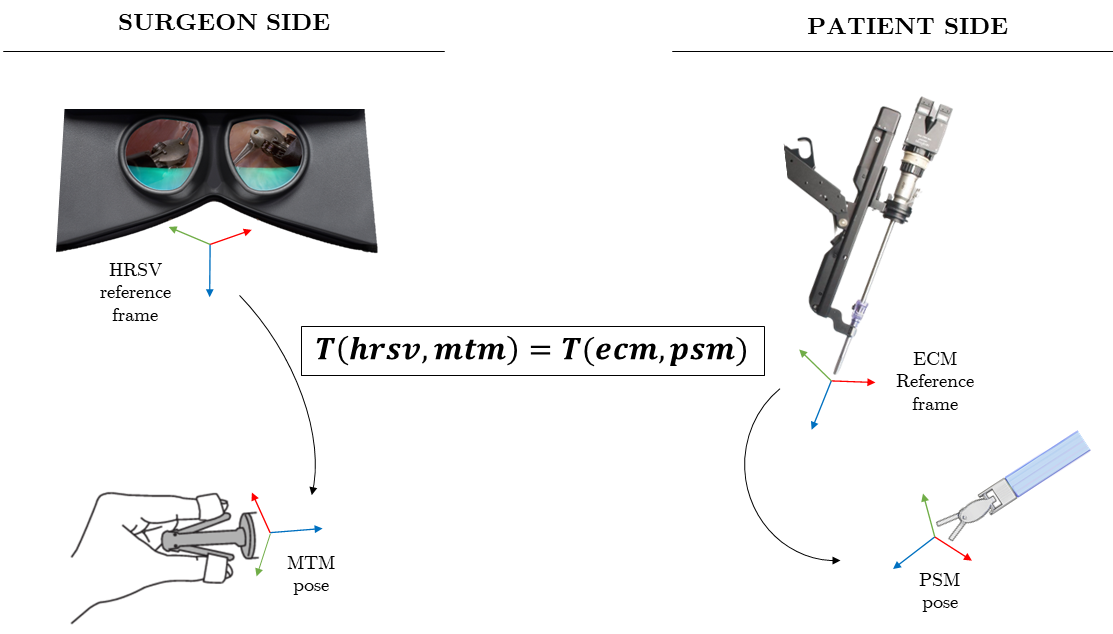
\includegraphics[width=\textwidth]{images/console_to_cart_transform.png}
    \caption{The equivalence of transformations between the console space and the surgical space. The transformation matrix that expresses the pose of the manipulator in the \hrsv reference frame is used to compute the desired pose of the \psm in the \rf of the endoscope camera.}
    \label{fig:consoletocarttransform}
\end{figure}

In the real surgical context, the motors are used to automatically position the manipulators at the start of the procedure, for gravity compensation and for exploiting the redundancy of the kinematic chain to optimally position the links of the \mtm in order to avoid collisions with the surgeon's wrist. However, the same dynamic model used for these purposes can be exploited to apply assistive mechanical forces to the manipulators, the direction and magnitude of which are determined from the pose of the \psms's tooltip in the surgical \rf. A force to be applied to the manipulator tooltip is converted to the set of torques to be applied at each joint by the respective actuators. The parameters of this inverse dynamics model \cite{Fontanelli2017} for the generic i-\textit{th} link are:
\begin{itemize}
  \item The mass $m_i$ of the link
  \item The three components of the first moment $\textbf{m}_i$ of the link
  \item The six independent elements of the inertia tensor $\textbf{I}_i$ of the link
  \item The static and viscous coefficients of the link, $F_{s,i}$ and $F_{v,i}$ respectively
\end{itemize}

The \vf force computed in the virtual surgical space - in the simulator - is therefore converted, in real-time, to a set of 7 torques to be communicated as a ROS message to the \mtms. 
The same inverse dynamics model converts a torque to be applied to the end effector into a set of 7 torques to be applied to the joint motors. 

\subsection{Error Mapping}
Most of the assistance strategies implemented here will use the distance from the \psm to the target or obstacle as the primary metric for determining the intensity of the feedback force or torque. However, different surgical tasks and situations require a level of control over how the distance is taken into account. For this reason a sigmoidal mapping function is employed for the normalization of the linear or angular error into a suitable interval. Specifically, such mapping is formulated as:

\begin{equation}
  f_{map}(x) = \frac{1}{1+e^{5\delta w(x-t-h)}}
  \label{eq:sigmoidalmap}
\end{equation}

with $\delta = +1$ for guidance \vfs and $\delta = -1$ for avoidance \vfs ($\delta$ determines if the function increases or decreases monotonically). Here:
\begin{itemize}
  \item $t$ is the fixture \textit{threshold}, hence the value at which the sigmoid starts to significantly increase from zero
  \item $h$ is the distance from the threshold at which \textit{half} of the maximum force is provided
  \item $w$ controls the \textit{width} of the linear region, hence the steepness of the curve 
\end{itemize}
For example, if $t=2\si{mm}$ and $h=3\si{mm}$ the surgeon will start to feel a force for errors higher than 2\si{mm}, and at 5\si{mm} he will experience half of the maximum force that can be delivered.

\begin{figure}[h!]
  \centering
      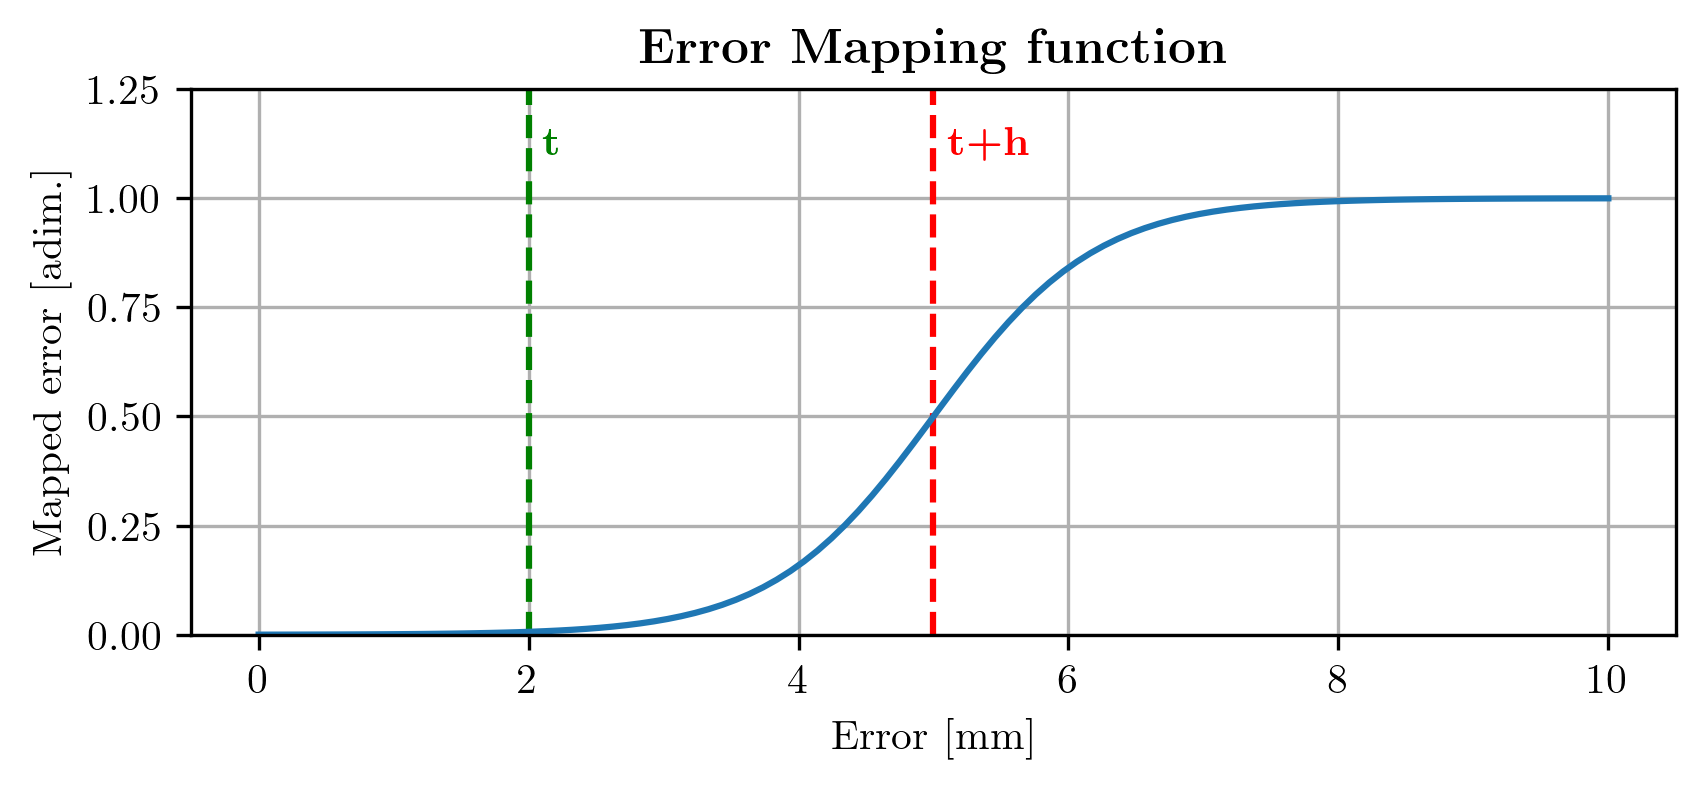
\includegraphics[width=0.75\textwidth]{images/mappingfunction.png}
      \caption{Plot of the Error Mapping function. The position of$t$ and $t+h$ can be set manually to achieve a suitable behavior of the assistance strategy. The x-axis refers to a generic error shown in millimeters, but the same mapping function can be applied to an angular error.} 
      \label{fig:mappingfunctiion}
\end{figure}

$t$, $h$ and $w$ are set manually in order to achieve an optimal "feeling" of the \vf. Their values, different from task to task, are reported in Tab.\ref{tab:thwvalues}.

\begin{table}
    \centering
    \caption{Error mapping parameters for the different tasks. \textit{Exchange}, \textit{Liver Resection} and \textit{Suturing} map both the distance error and the angular error, so the values of both mapping functions are reported.}
    \begin{tabular}{||c||c|c|c||}
        \hline
        \textbf{Task} & $\textbf{t} $ & $\textbf{h}$ & $\textbf{w}$ \\
        \hline\hline
        Path            & 2 mm & 2 mm & 500 \\ 
        \hline
        Rings           & 2 mm & 2 mm & 500 \\ 
        \hline
        Pillars         & 0.5 mm & 1 mm & 1000 \\ 
        \hline
        Exchange (distance)        & 3 mm & 2 mm & 500 \\ 
        \hline
        Exchange (angular)        & 5$^{\circ}$  & 5$^{\circ}$ & 2 \\ 
        \hline
        Thymectomy      & 0.5 mm & 1 mm & 1000 \\ 
        \hline
        Nephrectomy     & 2 mm & 2 mm & 500 \\ 
        \hline
        Liver Resection (distance) & 2 mm & 5 mm & 200 \\ 
        \hline
        Liver Resection (angular) & 5$^{\circ}$ & 15$^{\circ}$ & 1\\ 
        \hline
        Suturing (distance) & 1 mm & 3 mm & 300 \\ 
        \hline
        Suturing (angular) & 5$^{\circ}$ & 5$^{\circ}$ & 2\\ 
        \hline
    \end{tabular}
    \label{tab:thwvalues}
\end{table}

\subsection{Virtual Fixtures Algorithms}
As stated previously the force feedback delivered at the level of \mtm is computed, in terms of magnitude and direction, from the surgical space and therefore based on the relative position and orientation of the \psm's tooltip with respect to the objects in the virtual surgical scene. The simulator features 4 assistance algorithms implementing 4 different declinations of haptic assistance. Different algorithms are deployed inside specific surgical tasks based on the task morphology and goals:
\begin{itemize}
  \item \textbf{Trajectory Guidance:} This algorithm outputs a force vector that assists the surgeon in following a pre-defined 3D trajectory. A visco-elastic force pulls the \ee tooltip toward the closest point of the trajectory, and a visco-elastic torque aligns the tooltip's orientation with the trajectory tangent vector, computed at the closest point.
  \item \textbf{Obstacle Avoidance:} An Obstacle Avoidance algorithm prevents the practitioner from colliding with the virtual objects in the scene, which may represent, for example, delicate anatomical structures that must not be touched during surgery. A visco-elastic force is, therefore, applied to the \ee tooltip in order to push it away from the closest point of the obstacle.
  \item \textbf{Insertion Guidance:} Some surgical tasks require the insertion of the instrument's tooltip into a narrow space. This algorithm, from an initial position of the \psm and a target position, aids the surgeon in approaching the target on an optimal insertion path, without deviating from it.
  \item \textbf{Surface Guidance:} After defining, in the pre-operative stage, an ideal surface of operation (the surface can be of any morphology and should be defined as a mesh of points), a Surface Guidance algorithm generates forces and torques that keep the surgical tool on such surface and with an orientation tangent to it. 
\end{itemize} 
Table \ref{tab:taskswithvfs} highlights which of these \vf algorithms are used in each of the task featured in the simulator.
\begin{table}
    \caption{The surgical tasks featured in the simulator and the virtual fixtures algorithms used for each of them. Although the modular implementation of the simulator allows to include multiple \vf algorithms in a single task (multiple-steps executions will be included in the future), for this study only one \vf algorithm is used per task.}
    \centering
    \begin{tabular}{||c|c||}
        \hline
        \textbf{Path} & \textit{Trajectory Guidance} \\
        \hline
        \textbf{Rings} & \textit{Insertion Guidance} \\
        \hline
        \textbf{Pillars} & \textit{Obstacle Avoidance} \\
        \hline
        \textbf{Exchange} & \textit{Trajectory Guidance} \\
        \hline
        \textbf{Thymectomy} & \textit{Obstacle Avoidance}  \\
        \hline
        \textbf{Nephrectomy} & \textit{Insertion Guidance} \\
        \hline
        \textbf{Liver Resection} & \textit{Surface Guidance} \\
        \hline
        \textbf{Suturing} & \textit{Trajectory Guidance} \\
        \hline
    \end{tabular}
    \label{tab:taskswithvfs}
\end{table}
Figure \ref{fig:vfsgraphics} graphically illustrates the \vf algorithms as described above, but a detailed analytical formulation of each algorithm follows in the next sections.

\begin{figure}
    \centering
    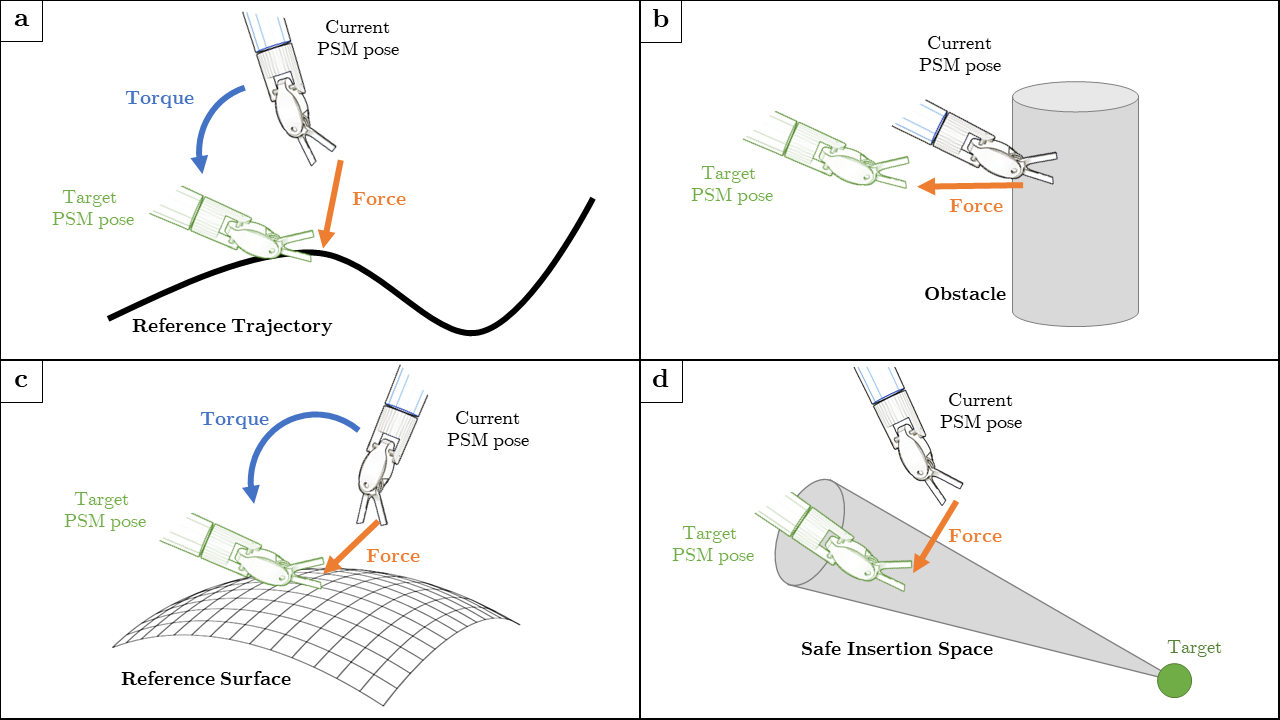
\includegraphics[width=\textwidth]{images/vfs_graphics.png}
    \caption{Graphics scheme of the 4 virtual fixtures featured as assistance strategies in the surgical simulator. \textbf{a.} Trajectory Guidance; \textbf{b.} Obstacle Avoidance; \textbf{c.} Surface Guidance; \textbf{d.} Insertion Guidance. A representative \psm's pose is shown, and a target pose is also depicted in a green hue, together with the force (orange arrows) and torque (blue arrows) that will guide the motion toward the target pose.}
    \label{fig:vfsgraphics}
\end{figure}

\paragraph{Trajectory Guidance} 
Considering a generic three-dimensional reference trajectory planned in the pre-operative stage, the feedback forces will be calculated according to the relative position and orientation of the trajectory itself and the tooltip reference frame. Both the forces and torques are computed in real-time as the sum of an elastic and a viscous contribution: while the elastic component accounts for the positional or angular error to the closest point of the reference trajectory - and the tangent computed in such point, accordingly - the viscous components are proportional to the temporal rate of change of the errors themselves. 

A viscoelastic model allows to achieve a guidance and error-compensating assistance that is less prone to overshooting behaviors and to oscillations. Moreover, with the force and torque calculated as 
\begin{equation}
    \vect{F} = k_F\cdot\vect{F}_{elastic} + \eta_F\cdot\vect{F}_{viscous} 
    \label{eq:force}
\end{equation}
\begin{equation}
    \vect{T} = k_T\cdot\vect{T}_{elastic} + \eta_T\cdot\vect{T}_{viscous}
    \label{eq:torque}
\end{equation}
one tunes the elastic gains $k_F$ and $k_T$ and the viscous damping coefficients $\eta_F$ and $\eta_T$ in order to achieve a comfortable balance between the components and a stable behavior of the feedback force, which may vary from operator to operator, as well as from task to task.

\begin{figure}
    \centering
    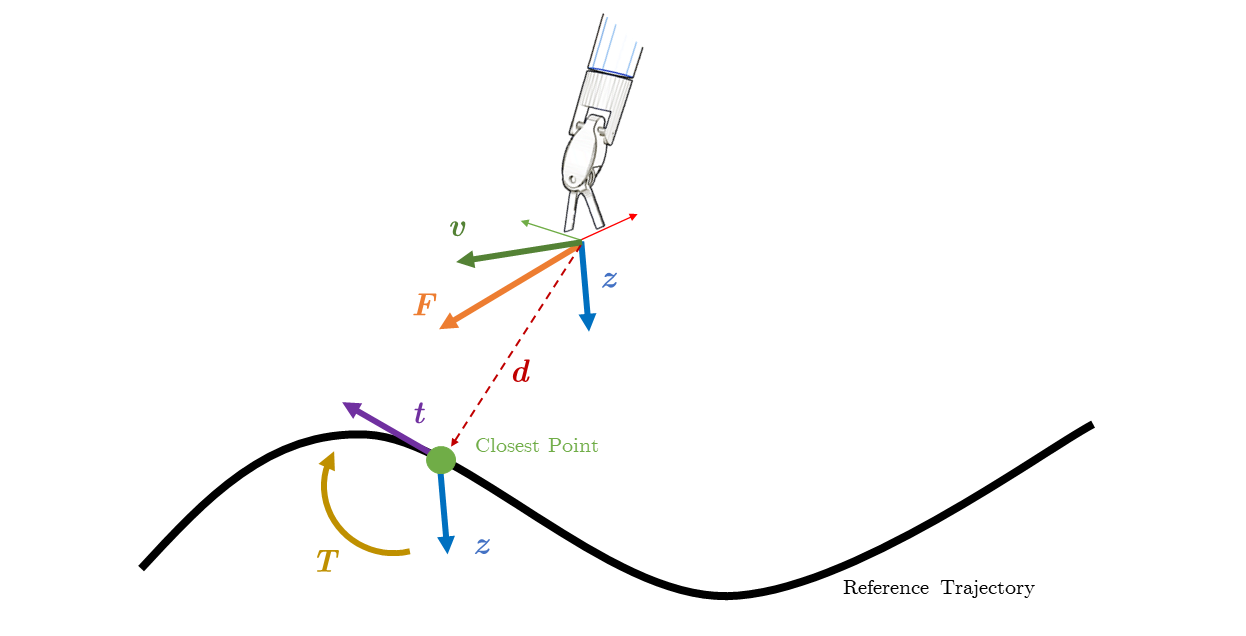
\includegraphics[width=0.8\textwidth]{images/trajectory_guidance.png}
    \caption{Vectors involved in the computation of the Trajectory Guidance \vf. The \psm is shown in an example representative pose with respect to the reference trajectory.}
    \label{fig:trajectoryguidance}
\end{figure}

Figure \ref{fig:trajectoryguidance} illustrates the vectors involved in the computation of the virtual fixture; specifically, contributions in Equation \ref{eq:force} expanded as:
\begin{equation}
    \vect{F}_{elastic} = f_{map}(\|\vect{d}\|)\cdot\frac{\vect{d}}{\vect{d}}
\end{equation} 
\begin{equation}
    \vect{F}_{viscous} = 
    \begin{cases} 
        \vect{d}, & \textit{if         } \vect{v}\cdot\vect{d}<0 \\
         \texttt{rotate}(\vect{v},\theta,\vect{r}), & \textit{otherwise}
    \end{cases}
\end{equation} 

Here, $\vect{d}$ is the distance vector going from the surgical instrument to the closest point in the trajectory, $\vect{v}$ is the velocity of the surgical instrument, while $\theta$ and $\vect{r}$ are the angle and axis of rotation which will align the velocity vector $\vect{v}$ with $\vect{d}$, respectively:
\begin{equation}
    \theta = (1+\vect{v}\cdot\vect{d})\cdot\frac{\pi}{2}
\end{equation}
\begin{equation}
    \vect{r} = \vect{v}\times\vect{d}
\end{equation}
This implementation is adapted from \cite{Enayati2016}. Similarly, contributions to the torque (Equation \ref{eq:torque}) are expanded as: 
\begin{equation}
    \vect{T}_{elastic} = \arccos (\vect{z}\cdot\vect{t} ) \cdot \vect{z} \times \vect{t}
    \label{eq:telastic}
\end{equation}
\begin{equation}
    \vect{T}_{viscous} = \frac{d}{dt} \left[ \arccos (\vect{z}\cdot\vect{t} ) \right] \cdot \vect{z} \times \vect{t}
    \label{eq:tviscous}
\end{equation}
The role of the torque is to align the z-axis of the surgical tool's reference frame with the tangent of the trajectory $\vect{t}$ at its closest point. In Equation \ref{eq:telastic} and Equation \ref{eq:tviscous}, the angle and axis of rotation which will achieve this alignment are $\arccos(\vect{z}\cdot\vect{t})$ and $\vect{z} \times \vect{t}$, respectively.

\begin{figure}
    \centering
    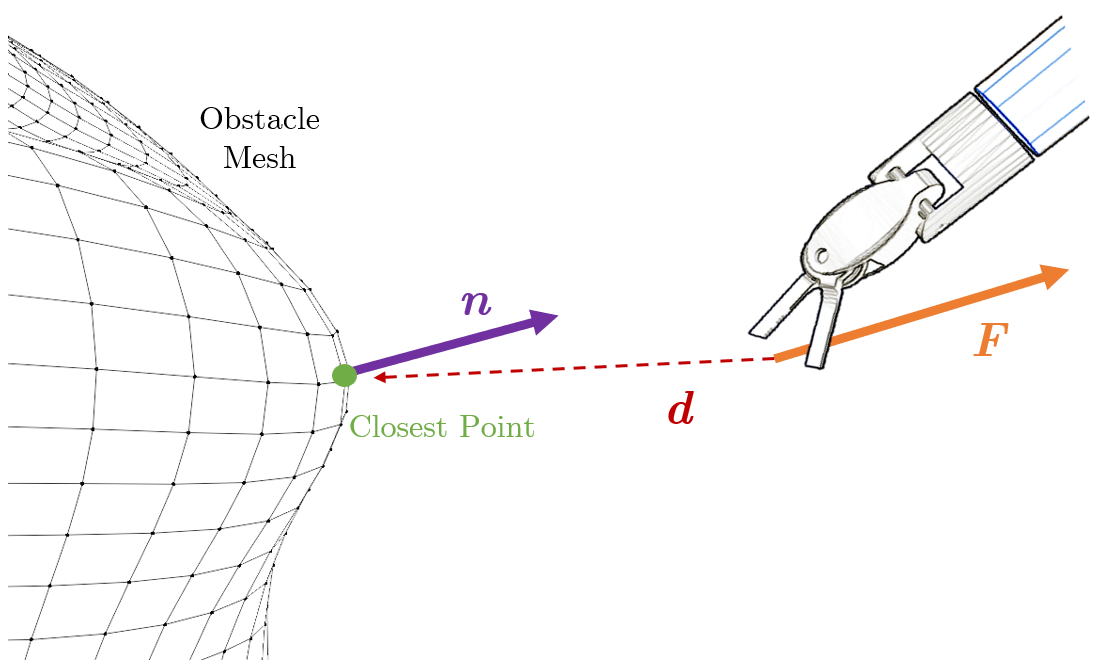
\includegraphics[width=0.6\textwidth]{images/obstacle_avoidance.png}
    \caption{Vectors involved in the computation of the Obstacle Avoidance \vf. The \psm is shown in an example representative pose with respect to the obstacle mesh.}
    \label{fig:obstacleavoidance}
\end{figure}

\paragraph{Obstacle Avoidance} The format for representing 3D objects in the simulator developed for this work is \texttt{stl} (Standard Triangle Language): in this format, a solid is defined as a list of 3D spatial coordinates of vertex points and a list of edges connecting them in groups of 3. Under a different light, an \texttt{stl} solid is a group of triangles, or ``subsurfaces'', sharing sides: the \texttt{stl} format also embeds a list of unique vector normals, one for each triangle, useful for easily accessing the orientation of each. The closest vertex point to the \psm's tooltip is identified and, with $\vect{d}$ as the normalized distance vector going from such point to the tooltip and $\vect{n}$ as the normal vector of the object mesh at that point (a graphic representation is depicted in Figure \ref{fig:obstacleavoidance}), the force is again computed as the sum of an elastic component, modulated by $k$, and a viscous one, modulated by $\eta$:
\begin{equation}
    \vect{F} = \left[k\cdot f_{map}(\|\vect{d}\|) + \eta\cdot \frac{d}{dt} \left( f_{map}(\|\vect{d}\|)\right)\right]\cdot \frac{\vect{n}}{\|\vect{n}\|} 
    \label{eq:obstacleavoidancef}
\end{equation}
$k$ and $\eta$ can be adjusted while performing the task and the visco-elastic balance will change accordingly, in real-time. Here, the addition of a viscous component was suggested by clinical experts, as the elastic-only model was felt ``jelly-like'' and, in a few cases, oscillating. $f_{map}(\cdot)$ is the error mapping function with $\delta=-1$With the addition of the viscous component, the same clinicians confirmed a more appropriate behavior of the assistance force.


It is to be highlighted that, for meshes with particularly sharp edges, the normal vector $\vect{n}$ at the closest point may not be optimally defined: in Figure \ref{fig:normalsaveraging} (left), the closest point normals is directed upwards, which is not necessarily the motion direction that maximizes the distance with the \psm's tooltip. To solve this, instead of defining the normal vectors at the centerpoint of each subsurface, the normals taken into consideration are defined at the vertex points and are computed as the average of the normals of the subsurfaces that share the vertex point. This is illustrated in Figure \ref{fig:normalsaveraging} (right), where it's also evident how the direction of the force generated in this case actually maximizes the distance with the \ee. With this adjustment, the spatial distribution of normal vectors is smoothed and so is the force field generated by the obstacle avoidance module.
\begin{figure}
    \centering
    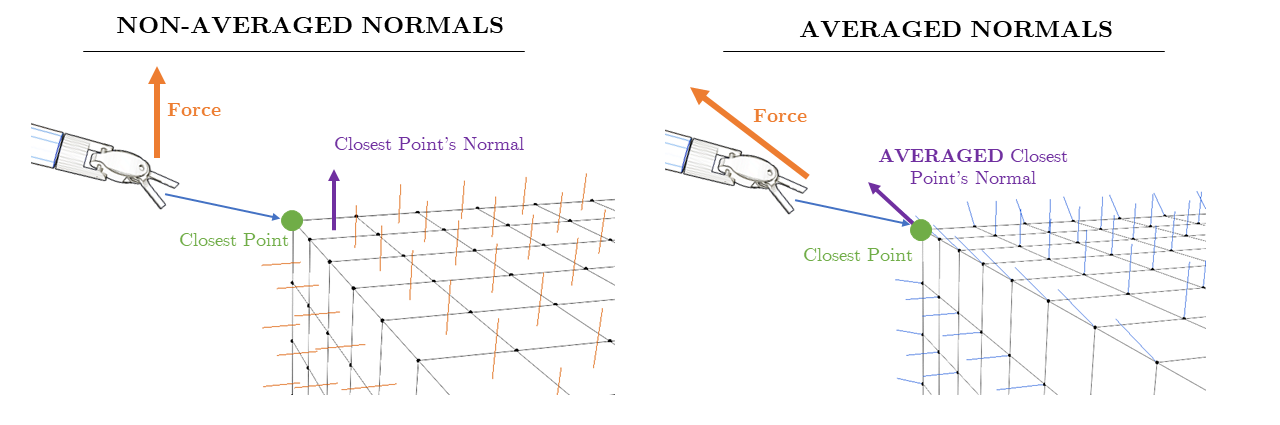
\includegraphics[width=\textwidth]{images/normals_averaging.png}
    \caption{On the left, the assistance force is generated from the non-averaged normals, defined at the subsurface centerpoints. On the right, the assistance force is generated from the averaged normals, defined at the vertices. In this figure, the mesh is composed of 4-vertices ``quads'', but the same concept holds to meshes with subsurface triangles.}
    \label{fig:normalsaveraging}
\end{figure}
Numerically, if a vertex is shared among $S$ subsurfaces, the averaged normal vector $\hat{\vect{n}}$ at that vertex is computed as:
\begin{equation}
    \hat{\vect{n}} = \frac{1}{S}\sum_{i=1}^{S} \vect{n}_i
    \label{eq:normalsaveraging}
\end{equation}

\begin{figure}
    \centering
    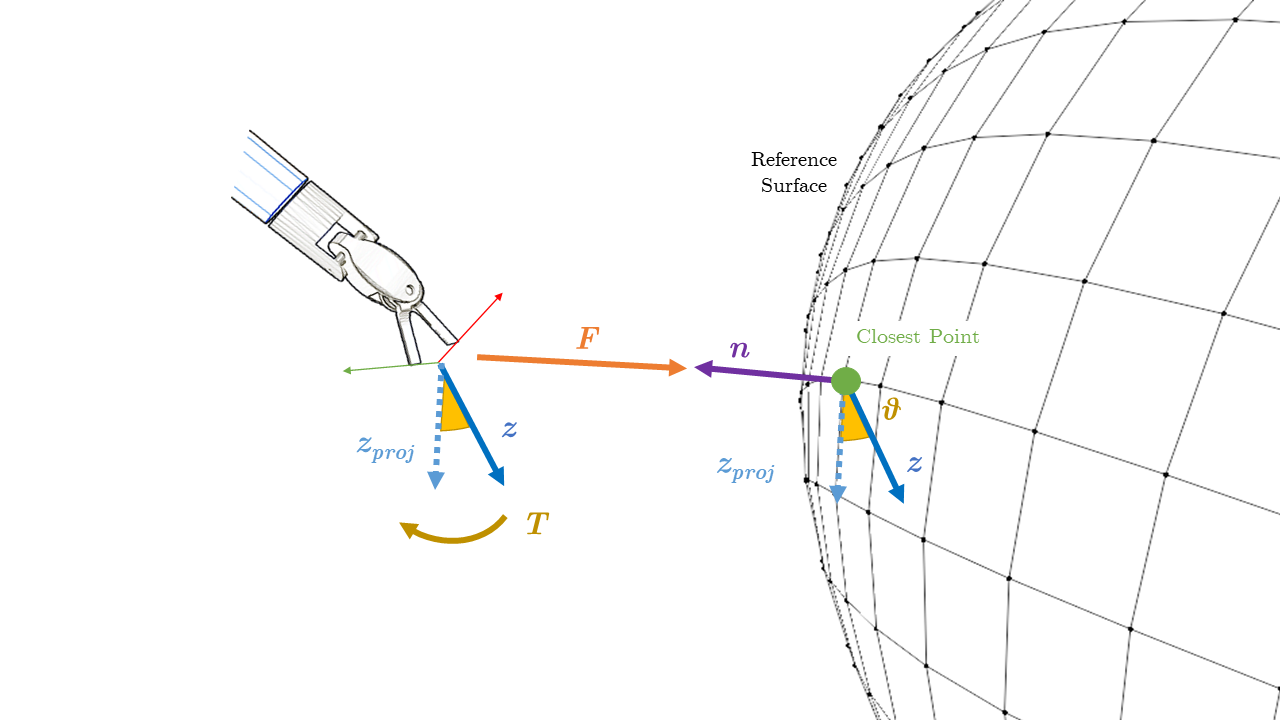
\includegraphics[width=0.8\textwidth]{images/surface_guidance.png}
    \caption{Vectors involved in the computation of the Surface Guidance \vf. The \psm is shown in an example representative pose with respect to the surface mesh.}
    \label{fig:surfaceguidance}
\end{figure}

\paragraph{Surface Guidance} Similarly to the Obstacle Avoidance algorithm, an \texttt{stl} surface may be used in some context as a reference for guidance: this implementation indeed computes a force and a torque that attracts and align the surgical \ee toward the surface itself. 

The force is computed with the same logic as in the Obstacle Avoidance algorithm, with the distance vector $\vect{d}$ from the \psm tooltip to the closest point of the surface mesh, and $\vect{n}$ the normal vector of the surface at that point. However, in the error mapping function $f_{map}(\cdot)$ the value of $\delta$ is set to $+1$ and the curve increases monotonically, so that the force is always attractive and is highest when the \psm is furthest from the surface mesh. The formula for the force is:

\begin{equation}
    \vect{F} = \left[k_F\cdot f_{map}(\|\vect{d}\|) + \eta_F\cdot \frac{d}{dt} \left( f_{map}(\|\vect{d}\|)\right)\right]\cdot \frac{\vect{-n}}{\|\vect{n}\|} 
\end{equation}

Compared to Equation \ref{eq:obstacleavoidancef}, the sign of the normal vector $\vect{n}$ is inverted.

To compute the torque, one considers the relative orientation of the $\vect{z}$-axis of the \psm's tooltip reference frame and the normal vector $\vect{n}$ at the closest point on the surface. In particular, the torque generated on the manipulator will aim at aligning the $\vect{z}$-axis with its projection on the tangent plane of the surface, defined by the normal vector $\vect{n}$ at the closest point. The vector projection on the tangent plane is the difference between the vector itself and its projection on the normal vector $\vect{n}$, obtained from the dot product operator:
\begin{equation}
    \vect{z}_{proj} = \vect{z} - (\vect{z}\cdot\vect{n})\vect{n}
\end{equation} 

From this, the torque is again the sum of an elastic component dependent on the angle $\theta$ between $\vect{z}$ and $\vect{z}_{proj}$ (specifically $\theta = \arccos(\vect{z}\cdot\vect{z}_{proj})$) , and a viscous one proportional to the angle's derivative in time. The formula for the torque is
\begin{equation}
    \vect{T} = \left[k_T\cdot f_{map}(\theta) + \eta_T\cdot \frac{d}{dt} \left( f_{map}(\theta)\right)\right]\cdot \frac{\vect{z} \times \vect{z}_{proj}}{\|\vect{z} \times \vect{z}_{proj}\|}
    \label{eq:}
\end{equation}

where $\vect{z} \times \vect{z}_{proj}$ is the axis of rotation.

The surface mesh is submitted to the same smoothing procedure as the obstacle mesh (Figure \ref{fig:normalsaveraging}, Equation \ref{eq:normalsaveraging}).




\paragraph{Insertion Guidance} From a starting pose and a target object it's possible to define an \textit{insertion cone} that defines a safe space for the \ee to move while approaching the target object. An insertion angle $\alpha$ determines the conical aperture and, therefore, how narrow the safe space is as the tooltip gets closer to the target. The vector $\vect{\textdelta}$ links the initial \psm position to the target. 

\begin{figure}
    \centering
    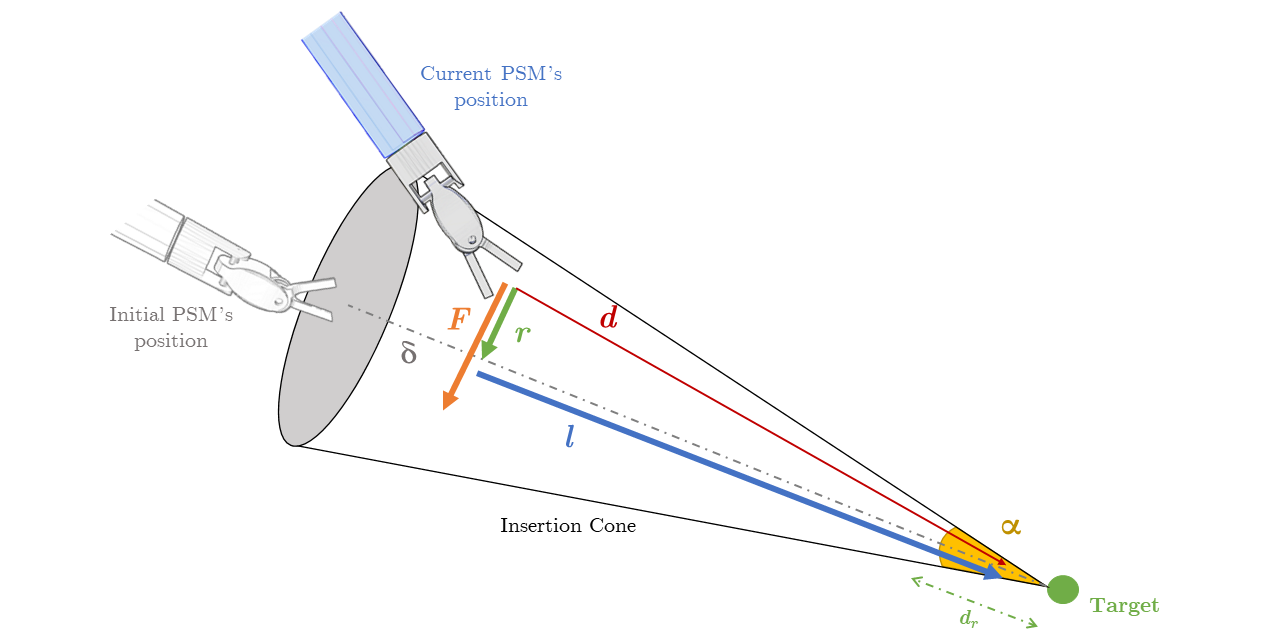
\includegraphics[width=0.8\textwidth]{images/insertion_guidance.png}
    \caption{Vectors involved in the computation of the Insertion Guidance \vf. The \psm is shown in a ``current'' example representative pose with respect to the insertion cone, which is defined from the initial \psm position and the target position.}
    \label{fig:insertionguidance}
\end{figure}

The position of the \ee in its longitudinal and radial components with respect to the reference insertion cone, $\vect{l}$ and $\vect{r}$ respectively, as follows:

\begin{equation}
    \vect{l} =  \left(\vect{d}\cdot \frac{\vect{\textdelta}}{\|\vect{\textdelta}\|} \right) \frac{\vect{\textdelta}}{\|\vect{\textdelta}\|}
\end{equation} 
\begin{equation}
    \vect{r} = \vect{d} - \vect{l}
\end{equation}

Figure \ref{fig:insertionguidance} shows a representative example for the calculations of the Insertion Guidance \vf force, and the vectors involved.

For the insertion cone, fixed in space, the aperture $a$ relates the longitudinal and radial components through the angle $\alpha$ (expressed in degrees) as follows:
\begin{equation}
    a = \tan\left(\alpha\cdot\frac{\pi}{180}\right)
\end{equation}
\begin{equation}
    \|\vect{r}\| = \|\vect{l}\|\cdot a
\end{equation}


The computed feedback force aims at maintaining the \ee position inside the safe insertion cone, therefore the threshold in the error mapping function $f_{map}(\cdot)$ is set to $t = \|\vect{r}\|$, the value of which varies over time and depends on the longitudinal coordinate $\|\vect{l}\|$. When the tooltip of the surgical instrument is very close to the target, the threshold becomes very small and the force gets very close to the maximum value very rapidly, which causes instabilities. To solve this issue, a ``relax distance'' $d_r$ is introduced: when the \ee is close enough to the target, the force is relaxed and scaled down to half of its value to interfere less with the surgeon's motion so close to the target. A clinical expert suggested that $d_r$ should be 20\% of the height of the cone. Considering this adjustment, the force feedback for the Insertion Guidance assistance strategy is:
\begin{equation}
    \vect{F} = r(\|l\|)\left[k\cdot f_{map}(\|\vect{a}\|) + \eta\cdot \frac{d}{dt} \left( f_{map}(\|\vect{a}\|)\right)\right]\cdot \frac{\vect{a}}{\|\vect{a}\|}
    \label{eq:insertionguidance}
\end{equation}

with

\begin{equation}
    r(\|l\|) = 
    \begin{cases}
        1 & \text{if } \|l\| > d_r \\
        0.5 & \text{if } \|l\| \leq d_r
    \end{cases}
\end{equation}

scaling the force down to its relaxed value depending on the insertion depth. As per all the other assistance algorithms, $k$ and $\eta$ control the PD gains of the force feedback and are set manually by the practitioner, who is also able to adjust them in real-time.

A similar implementation of this \vf, from which this algorithm is inspired, was proposed by Bettini \textit{et al.} \cite{Bettini2004}.

\section{Clinical Validation}
\label{sec:clinicalvalidation}
Two resident surgeons from the \textit{Istituto Europeo di Oncologia} (Milano, MI, Italy), both regularly performing \ac{ramis} procedures with the \textit{daVinci}\cright robot, kindly dedicated their time for testing the surgical simulator in all its aspects, from the motion truthfulness to the complexity of the wrist articulation to the invasiveness and visco-elastic balance of the virtual fixtures. Their opinion and expertise were precious and insightful tools that guided the development toward a clinically validated robotic surgical simulator. 
Moreover, the most expert resident surgeon allowed to have his performance recorded when practicing with the simulator, which will be considered ``peak performance'' in the experimental analysis. 

\begin{figure}
    \centering
    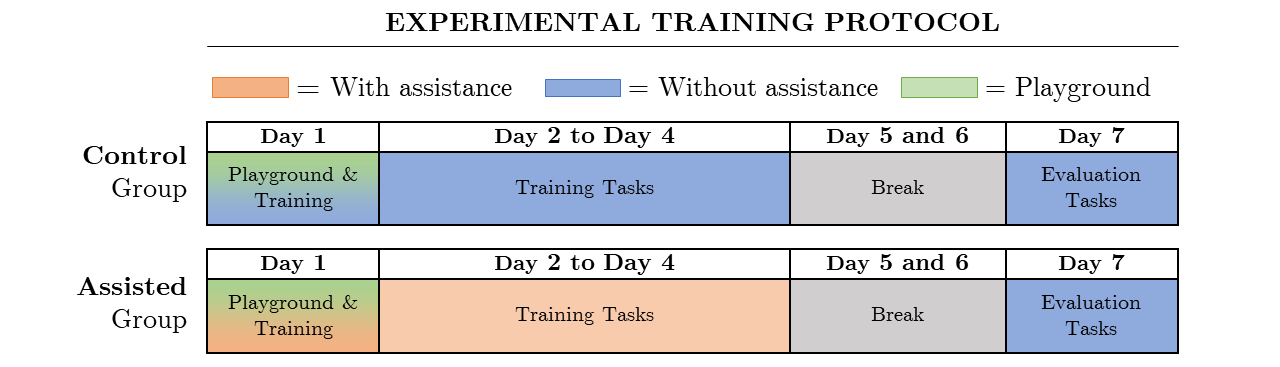
\includegraphics[width=\textwidth]{images/training_protocol.png}
    \caption{Schematic of the training protocol applied to the subject undergoing the experimental phase. On the days highlighted in orange, the \vf assistance was provided to the group indicated; on the days highlighted in blue, the subjects were not assisted by \vfs. In green, the \textit{Playground} environment is a propedeutic task shown on the first day only, to familiarize the subjects with the simulator and the \davinci system.}
    \label{fig:trainingprotocol}
\end{figure}
\section{Experimental Protocol}
In order to assess the effectiveness and benefits of the developed assistance strategies and the simulator they have been implemented in, an experimental study was conducted on a group of novice users interfacing with the simulated surgical environment. 

A group of 8 volunteers was asked to execute the surgical tasks implemented in the simulator over multiple repetitions: some of the subjects were assisted with the \vf algorithms described in the previous paragraphs, and others performed the tasks without any haptic assistance. Considering that the scope is to evaluate the role of haptic assistance in the learning process, the program was carried out over the course of a week in order to appreciate a possible variation in performance, which does not usually occur in the context of learning surgical skills.
The 8 volunteers participating in the study were divided into 2 groups:
\begin{itemize}
    \item An \textbf{Assited Group} (Group A) of 4 subjects, who received haptic assistance while performing the tasks.
    \item A \textbf{Control Group} (Group C) of 4 subjects, who were not assisted by \vfs while teleoperating.
\end{itemize}

Subjects were 25\% females and 75\% males, between 23 and 27 years of age, all right-handed and either had never teleoperated a surgical robot or did it less than 5 times. Assignation to the control or assisted group was random.

The subjects underwent a week-long training phase:
\begin{itemize}
  \item On \textit{Day 1}, they were given a concise explanation about the \textit{daVinci}\cright surgical system, the simulator, haptics, and the training protocol. Later, each subject experienced 5 minutes in a \textit{Playground} environment (Figure \ref{fig:taskspanel}), purposely designed to understand the elementary mechanics of teleoperation, clutching and object grasping. No performance metric was recorded at this time
  \item From \textit{Day 1} to \textit{Day 4}, after familiarizing with the \textit{Playground}, they were asked to execute the four training tasks of the simulator (\textit{Path, Rings, Pillars} and \textit{Exchange}), each one for a total of 3 repetitions. Tasks appeared sequentially in a random order, contributing to un-bias the results. Subjects in group A were assisted by the \vfs while training, while subjects in group C received no mechanical assistance force. At the beginning of each daily session, subjects could interact with the \textit{Playground} environment for 1 minute at maximum.  
  \item On \textit{Day 5} and \textit{Day 6} subjects were given a break period and no training was performed.
  \item On \textit{Day 7} they were asked to execute the four surgical evaluation tasks of the simulator (\textit{Thymectomy, Nephrectomy, Liver Resection} and \textit{Suturing}), each one for a total of 3 repetitions. Again, tasks appeared sequentially in a random order, contributing to unbiasing the results. On this day, neither group A nor group C was assisted by the \vf algorithms.
\end{itemize}
This training protocol is schematized in Figure \ref{fig:trainingprotocol}. 

Crucially, during the training phase of the first 4 days, the intensity of the haptic assistance was progressively decreased on a daily basis: each day, the magnitude of the maximum force and torque was reduced by 25\% with respect to the first day. On day 4, the maximum force and torque delivered by the \vf algorithms were $0.25\cdot F_{max}$ and $0.25\cdot T_{max}$, respectively. This progressive reduction in the intensity of the \vfs was performed to avoid the subjects to become too dependent on the assistance, which would have made the evaluation of the effectiveness of the \vfs more difficult.

The layout of the training phase was studied and developed with a focus on examining how an enhanced training phase influences performance in a real surgical scenario. This aspect is known as \textit{Skill Transfer} and it is crucial in the development of a surgical simulator which, no matter how realistic and true-to-life it is, will never be able to replicate the complexity of a real surgical environment. To compensate for this, the 4 evaluation tasks executed on the last day were never shown to the subjects during the first 6 days, thus allowing to study if and to what extent the skills learned with the training tasks were transferred to the evaluation tasks. Naturally, to ensure a correct comparison of skill transfer, no assistance was provided to the subjects in the assisted group while performing the evaluation tasks on the last day.

The 2-days break was, instead, introduced to indagate the \textit{Skill Retention} that may be introduced by augmented training: positive skill retention occurs if the performance drop caused by a break period is reduced compared to normal. In this case, it is of interest to understand if the haptic assistance provided during the training phase causes a decrease in the performance drop across the break period.

\section{Performance Metrics}   
The simulator keeps track in real-time of the pose of all the objects in the scene, as well as other relevant parameters that can be employed to quantify performance. In order to properly conduct a comparative study between the two groups, the execution of the subjects involved in the training phase was considered in relation to the execution of the expert clinicians, as in Section \ref{sec:clinicalvalidation}. Their expertise, the number of robotic surgeries in their curricula and their daily usage of a \davinci robot made it possible to consider their execution of the training and evaluation surgical tasks as ``peak performance''. Therefore, the quality of the execution of a subject is always considered in relation to the execution of expert clinicians.

A group of \textit{metrics} is recorded at each frame of the simulation and then logged automatically in a \texttt{.csv} file. The simulator begins and ends the metrics acquisition automatically, detecting if the user has begun interacting with the objects and tools as well as if he has reached the target. This level of automatization guarantees that the metrics are logged in the same way for all subjects, and prevents the introduction of human errors when deciding when to start and terminate the logging. The metrics are the following:
\begin{itemize}
    \item $D$: Distance error, from the \ee to the closest point of the target (trajectory, surface or object)
    \item $A$: Angular error, from the \ee to tangent vector in the closest point of the reference trajectory or to the tangent plane in the closest point of a surface
    \item $F$: Feedback force, computed from the \vf. The force is computed also for the subjects in the non-assisted control group, but it's not delivered during the operation
    \item $T$: Feedback torque, computed from the \vf. The torque is computed also for the subjects in the non-assisted control group, but it's not delivered during the operation
    \item $M$: Missed exchanges. When, in the bi-manual tasks, an object is dropped when passing it from the left \psm to the right, or vice versa
    \item $C$: Clutch time, the fraction of the total task time during which the clutch pedal was pressed for repositioning
\end{itemize}  

Such parameters are recorded and logged at every frame, and they are averaged at the time of task completion in order to obtain a single mean value that refers to the execution as a whole. Thus, a set of 6 averaged metrics is available for each task execution.

\begin{figure}
    \centering
    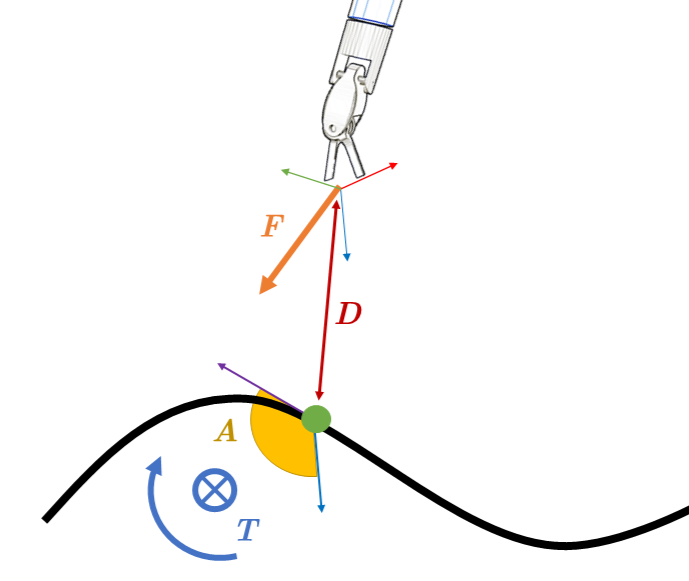
\includegraphics[width=0.6\textwidth]{images/metrics.png}
    \caption{Graphical representation of some of the performance metrics recorded during task execution. }
    \label{fig:metrics}
\end{figure}

As stated previously, in order to sensibly account a metric as a performance indicator for a comparative study, it must be normalized in relation to the execution of the expert clinicians. This is done by considering a \textit{relative metric} $\hat{X}$ as follows:
\begin{equation}
    \hat{X} = \frac{X_{subject}}{X_{expert}}
\end{equation}

The numerical value of performance is then established as a weighted average of the relative metrics. Depending on the surgical skills that each task requires, the weights are determined to reflect a resulting performance that properly accounts for the metrics themselves. The values of the weights in each task are reported in Table \ref{tab:performanceweights}

\begin{table}
    \caption{Weights assigned to the metrics in the computation of the performance score. The weight of a generic relative metric $\hat{X}$ is denoted as $w_{\hat{X}}$.}
    \centering
    \begin{tabular}{||c||c|c|c|c|c|c||}
        \hline
        \textbf{Task} & $w_{\hat{D}}$ & $w_{\hat{A}}$ & $w_{\hat{F}}$ & $w_{\hat{T}}$ & $w_{\hat{M}}$ & $w_{\hat{C}}$ \\
        \hline\hline
        \textit{Path}            & 3 & 2 & 3 & 1 & 0 & 1 \\
        \hline
        \textit{Rings}           & 5 & 0 & 4 & 0 & 0 & 1 \\
        \hline
        \textit{Pillars}         & 5 & 0 & 4 & 0 & 0 & 1 \\
        \hline
        \textit{Exchange}        & 2 & 2 & 2 & 1 & 2 & 1 \\
        \hline
        \textit{Thymectomy}      & 5 & 0 & 4 & 0 & 0 & 1 \\
        \hline
        \textit{Nephrectomy}     & 5 & 0 & 4 & 0 & 0 & 1 \\
        \hline
        \textit{Liver Resection} & 3 & 2 & 3 & 1 & 0 & 1 \\
        \hline
        \textit{Suturing}        & 2 & 3 & 1 & 2 & 1 & 1 \\
        \hline
    \end{tabular}
    \label{tab:performanceweights}
\end{table} 

If one defines the set of normalized metrics as $M = \left\{ w_{\hat{D}}, w_{\hat{A}}, w_{\hat{F}}, w_{\hat{T}}, w_{\hat{M}}, w_{\hat{C}}\right\}$, the numerical formulation for the performance score $P$ is:
\begin{equation}
    P = \frac{1}{10}\sum_{m\in M} w_{\hat{m}}\cdot\hat{m}
    \label{eq:performance}
\end{equation}

The value of $P$ gets closer to 1 if the performance of the subject is similar to the performance of the expert clinicians: in a few cases, some subjects recorded metrics that, when averaged, were better than the ones obtained from the execution of the surgeons. For this reason, in a few cases, the value of $P$ slightly exceeds 1.

During the experimental phase of this study, all the averaged metrics, the performance scores and the relative task, repetition and subjects were progressively logged and stored in a database: associating the performance to the subject and repetition allows to analyze its variations and trends.

% BIBLIOGRAPHY
% \bibliographystyle{unsrt}
% \bibliography{refs.bib}

\end{document}